\documentclass[a4paper,14pt, twoside, openright]{extreport}

\usepackage{times}
\usepackage{mathptmx}

\usepackage[utf8]{inputenc} 
\usepackage[T5]{fontenc} 
\usepackage[vietnamese]{babel}
 
\usepackage[bottom = 2.5cm, top = 2.5cm, inner= 3.5cm, outer = 2cm]{geometry}

\usepackage{amssymb, amsthm}
\usepackage[intlimits]{mathtools}
\usepackage{graphicx}

%\usepackage[colorlinks, breaklinks, pdfencoding=unicode]{hyperref}
%cho bản in
\usepackage{xcolor} % sử dụng khai báo màu
\usepackage[colorlinks, linkcolor = black, citecolor = black, urlcolor = black,  breaklinks, pdfencoding=unicode]{hyperref}

\usepackage[intoc]{nomencl}

\usepackage{indentfirst}% tạo indent ở đoạn đầu tiên 

\usepackage{fancyhdr}

\usepackage[defernumbers, backend=biber, style=numeric, citestyle = numeric-comp, sorting = nty]{biblatex} 
	\addbibresource{bibtex/biblio_vn.bib} 
	\addbibresource{bibtex/biblio_en.bib}

\usepackage{tikz}%ve hinh
\usetikzlibrary{calc}
\usepackage{eso-pic} 

\usepackage[toc]{appendix}

\usepackage{tocloft}

% các thông số của văn bản
\renewcommand{\baselinestretch}{1.3}
\setlength{\parindent}{1.27 cm}
\setlength{\parskip}{6pt}

% xoá các heading trên các trang trắng
\newcommand{\clearHeading}{%*\label{line:lvtotnghiep_definition_clearHeading}*)
	\clearpage	
	\pagestyle{empty}     
	\cleardoublepage
	\pagestyle{fancyplain}
}

% định dạng trang
\pagestyle{fancyplain} 
\renewcommand{\chaptermark}[1]{%
	\markboth{\sl \chaptername~\thechapter.~#1}{}}
\renewcommand{\sectionmark}[1]{%
	\markright{\sl \thesection.~#1}}
  
	\fancyhf{}
	\lhead[\fancyplain{}{\leftmark}]{}
	\rhead[]{\fancyplain{}{\rightmark}}
	\lfoot[\thepage]{}
	\rfoot[]{\thepage}

%% các định nghĩa sử dụng trong trang bìa
\makeatletter
\newcommand*{\@chuyennganh}{Chuyên ngành?}
\newcommand*{\chuyennganh}[1]{\gdef\@chuyennganh{#1}}

\newcommand*{\@maso}{Chương trình gì?}
\newcommand*{\maso}[1]{\gdef\@maso{#1}}

\newcommand*{\@nam}{Năm ?}
\newcommand*{\nam}[1]{\gdef\@nam{#1}}

\newcommand*{\@thayhuongdan}{Tên thầy hướng dẫn ?}
\newcommand*{\thayhuongdan}[1]{\gdef\@thayhuongdan{#1}}



% trang bìa
\renewcommand{\maketitle}{
\begin{titlepage}%

\newgeometry{top=2cm,bottom=2cm,left=2cm,right=2cm}	
	
\AddToShipoutPicture*{%	
\AtTextCenter{%
 \makebox(0,0)[c]{
 \begin{tikzpicture}
 \draw[line width = 4pt](0,0)rectangle(\textwidth+2*0.3cm,\textheight+2*0.3cm);
 \end{tikzpicture}
 }
}
}

 \begin{center}
		
 {\fontsize{13}{15.6}\selectfont 
 ĐẠI HỌC QUỐC GIA HÀ NỘI\\
\textbf{ TRƯỜNG ĐẠI HỌC KHOA HỌC TỰ NHIÊN}\\
	\rule{3cm}{1.pt}} 

	\vfill
	\textbf{\@author}
	\vfill
 
 	{\fontsize{18}{21.6}\selectfont \textbf{\MakeUppercase\@title}}
	 \vfill
 
	LUẬN VĂN THẠC SĨ KHOA HỌC
	\vfill
 	
     \textbf{Hà Nội - \@nam}
     
  \end{center}
 \end{titlepage}%
}



%% trang bìa phụ
\newcommand{\maketitleTrangphu}{
\begin{titlepage}%

\AddToShipoutPicture*{%	
\AtTextCenter{%
 \makebox(0,0)[c]{
 \begin{tikzpicture}
 \draw[line width = 4pt](0,0)rectangle(\textwidth+2*0.3cm,\textheight+2*0.3cm);
 \end{tikzpicture}
 }
 }
}

 \begin{center}
	
 {\fontsize{13}{15.6}\selectfont% 
 ĐẠI HỌC QUỐC GIA HÀ NỘI\\
 \textbf{TRƯỜNG ĐẠI HỌC KHOA HỌC TỰ NHIÊN}\\
	\rule{3cm}{1.pt}} 

	\vfill
	\textbf{\@author}
	\vfill
 
 	{\fontsize{18}{21.6}\selectfont \textbf{\MakeUppercase\@title}}
	 \vspace{\baselineskip}
   	
	 \begin{tabular}{ll}
     Chuyên ngành:&\@chuyennganh\\
     Mã số:            &\@maso\\
     \end{tabular}
   
   	\vspace{2\baselineskip}
   	
   	LUẬN VĂN THẠC SĨ KHOA HỌC
   	
  	\vspace{\baselineskip}
  	       
  	NGƯỜI HƯỚNG DẪN KHOA HỌC: \@thayhuongdan

  	 \vfill
   	 \vfill
     	
     \textbf{Hà Nội - \@nam}

  \end{center}
\end{titlepage}%
}
\makeatother
% use to make a border arround page and text area
\usepackage{tikz}%ve hinh
\usetikzlibrary{calc}
\usepackage{eso-pic} 

\AddToShipoutPicture{%
		\AtTextCenter{%
		\makebox(0,0)[c]{
		\begin{tikzpicture}
		\draw[color = green!30](0,0)rectangle(\textwidth,\textheight);
		\end{tikzpicture}
			}
		}
      
		\AtPageLowerLeft{% khung bao quanh trang văn bản
		\begin{tikzpicture}
  		\draw[color = red,line width = 1.5pt](0,0) rectangle (\paperwidth-1.4pt,\paperheight-1.4pt);
		\end{tikzpicture}
		}
 }
  

\title{Ứng dụng các phổ Gamma trong nghiên cứu cấu trúc hạt nhân 156GD}
\author{Đoàn Quang Tuyền}
\chuyennganh{Vật lý hạt nhân}
\maso{101.102.3}
\nam{2015}
\thayhuongdan{TS. Nguyễn Văn A}

\begin{document}  

\pagestyle{empty}
\lfoot[]{}
\rfoot[]{}

\maketitle

\cleardoublepage
\maketitleTrangphu

\chapter*{Lời cam đoan}

Trình bày nội dung của phần Lời cam đoan. Nội dung của phần này thường được trình bày trong 1 trang.


\clearHeading
 \lfoot[\thepage]{}
 \rfoot[]{\thepage}
 \setcounter{page}{1}

\makeatletter
\renewcommand{\cftmarktoc}{\markboth{\sl \@title}{\sl \contentsname}}
\makeatother
\tableofcontents
\clearHeading

\makenomenclature
\renewcommand{\nomname}{Danh mục các từ viết tắt và các ký hiệu toán học}
\makeatletter
	\markboth{\sl \@title}{\sl \nomname}%*\label{line:lvthacsi_main_nom_markboth}*)
\makeatother
\printnomenclature
\clearHeading

	\chapter*{Mở đầu}
\addcontentsline{toc}{chapter}{Mở đầu}
\makeatletter
	\markboth{\sl \@title}{\sl Mở đầu}
\makeatother

Nêu tính cần thiết của đề tài, ý nghĩa khoa học và thực tiễn của Đề tài
	\clearHeading
	
	\chapter{Tổng quan}
\label{ch:tongquan}

Các tia bức xạ $\gamma$ sẽ được ghi nhận thông qua quá trình tương tác với vật chất. Đặc tính điện từ của các tia bức xạ $\gamma$ cho phép các tia bức xạ này có thể tương tác với các điện tử. Nguyên lý ghi nhận các tia bức xạ $\gamma$ dựa trên hiện tượng ion hóa: Các tia bức xạ $\gamma$ sẽ chuyển một phần hoặc toàn bộ năng lượng cho các điện tử. Các điện tử tự do được tạo thành trong quá trình này sẽ tương tác với các nguyên tử gần đó để tạo các điện tử thứ cấp. Các điện tử này được ghi nhận để xác định năng lượng của các tia $\gamma$. Kết quả của việc ghi nhận là một xung điện tỷ lệ với năng lượng của tia $\gamma$ đã  bị mất trong môi trường do quá trình tương tác.%*\label{line:simplereport_cosolythuyet_text}*) 

\section{Hiệu ứng quang điện}%*\label{line:simplereport_cosolythuyet_sec}*) 
Ở năng lượng thấp ($<$ 200 keV), tương tác giữa photon với một tinh thể Germanium được thực hiện thông qua hiệu ứng quang điện. Trong trường hợp này năng lượng của photon được hấp thụ hoàn toàn bởi tinh thể Germanium. Xác suất tương tác được tính một cách gần đúng theo công thức \cite{bib_Knoll, bib_ghinhanbucxa, bib_vatlyhatnhanungdung}:%*\label{line:simplereport_cosolythuyet_text2}*) 

\begin{equation}%*\label{line:simplereport_cosolythuyet_equaBegin}*)  
	P_{ph}\approxeq k\cfrac{Z^{n}}{(h\nu)^{3.5}}
\label{equ:huquangdien}%*\label{line:simplereport_cosolythuyet_huquangdien}*) 
\end{equation}%*\label{line:simplereport_cosolythuyet_equaEnd}*)  

Trong đó, giá trị của $n$ thay đổi từ 4 đến 5 tương ứng với khoảng năng lượng của photon từ 0 đến 3 MeV, $h\nu$ \nomenclature{$\nu$}{Tần số sóng điện từ} và $Z$ lần lượt là năng lượng của photon và số hiệu nguyên tử của Germanium.%*\label{line:simplereport_cosolythuyet_text3}*) 

\section{Hiệu ứng Compton}

Công thức \ref{equ:huquangdien} được áp dụng cho các photon có năng lượng thấp, tuy nhiên khi photon có năng lượng lớn hơn ($\approx$ 200 keV đến 8 MeV), hiệu ứng Compton sẽ chiếm ưu thế. Trong quá trình này, một photon có năng lượng $h\nu_{0}$ sẽ thực hiện tương tác không đàn hồi với một điện tử\footnote{Cần phân biệt giữa tán xạ Compton với tán xạ Rayleigh trong đó các tia $\gamma$, sau khi tương tác với một điện tử, thay đổi hướng chuyển động và không mất đi năng lượng.}. Một phần năng lượng của photon bị mất do tương tác với điện tử và các tia $\gamma$ sau  đó sẽ tán xạ dưới một góc $\theta$ \nomenclature{$\theta$}{Góc tán xạ} so với hướng ban đầu với năng lượng $h\nu$. Theo định luật bảo toàn năng lượng và động lượng ta có: %*\label{line:simplereport_cosolythuyet_text4}*)
\begin{equation}
	h\nu=\cfrac{m_{0}c^{2}\alpha}{1+\alpha(1-\cos{\theta})}
\end{equation}

Trong đó $\alpha=\cfrac{h\nu_{0}}{m_{0}c^{2}}$, $m_{0}$ là khối lượng của điện tử. Động năng của điện tử $(T=h\nu_{0}-h\nu)$ đạt cực 	đại nếu $\theta=\pi$. Tiết diện phản ứng vi phân tính trên một điện tử $\sigma_{e}$ \nomenclature{$\sigma_e$}{Tiết diện phản ứng vi phân trên một điện tử} với một góc khối $\Omega$ được thể hiện bằng công thức Klein-Nishina \cite{bib_Klein}

\begin{equation}
\cfrac{d \sigma_{e}}{d \Omega} = \cfrac{r_{0}^{2}}{2} 
\biggl\{
 \cfrac{1}{[1+\alpha(1-cos\theta)]^{2}}
 \biggl [
	1+cos^{2}\theta+\cfrac{\alpha^{2}(1-cos\theta)^{2}}{[1+\alpha (1-cos\theta)]}
 \biggr ]
\biggr\}
\end{equation}

trong đó $r_{0}$\nomenclature{$r$}{Bán kính tán xạ của điện tử} bán kính của điện tử. 

Các giá trị tiết diện phản ứng vi phân đối với các photon có năng lượng từ 0.2 MeV đến 2 MeV (khoảng giá trị đặc trưng được sử dụng khi nghiên cứu phổ các tia bức xạ $\gamma$) được thể hiện trên Hình \ref{fig:klein}. Các giá trị đã được chuẩn hóa theo giá trị tiết diện phản ứng cực đại được tính theo hướng của photon. Ở mức năng lượng cao ($\geq$ 1 MeV) hầu hết các tia bức xạ $\gamma$ tán xạ ở một góc rất nhỏ. Tuy nhiên, ở năng lượng thấp, các tia $\gamma$ có thể tán xạ ở các góc lớn hơn. %*\label{line:simplereport_cosolythuyet_text5}*)

\begin{figure}[!h]
\centering
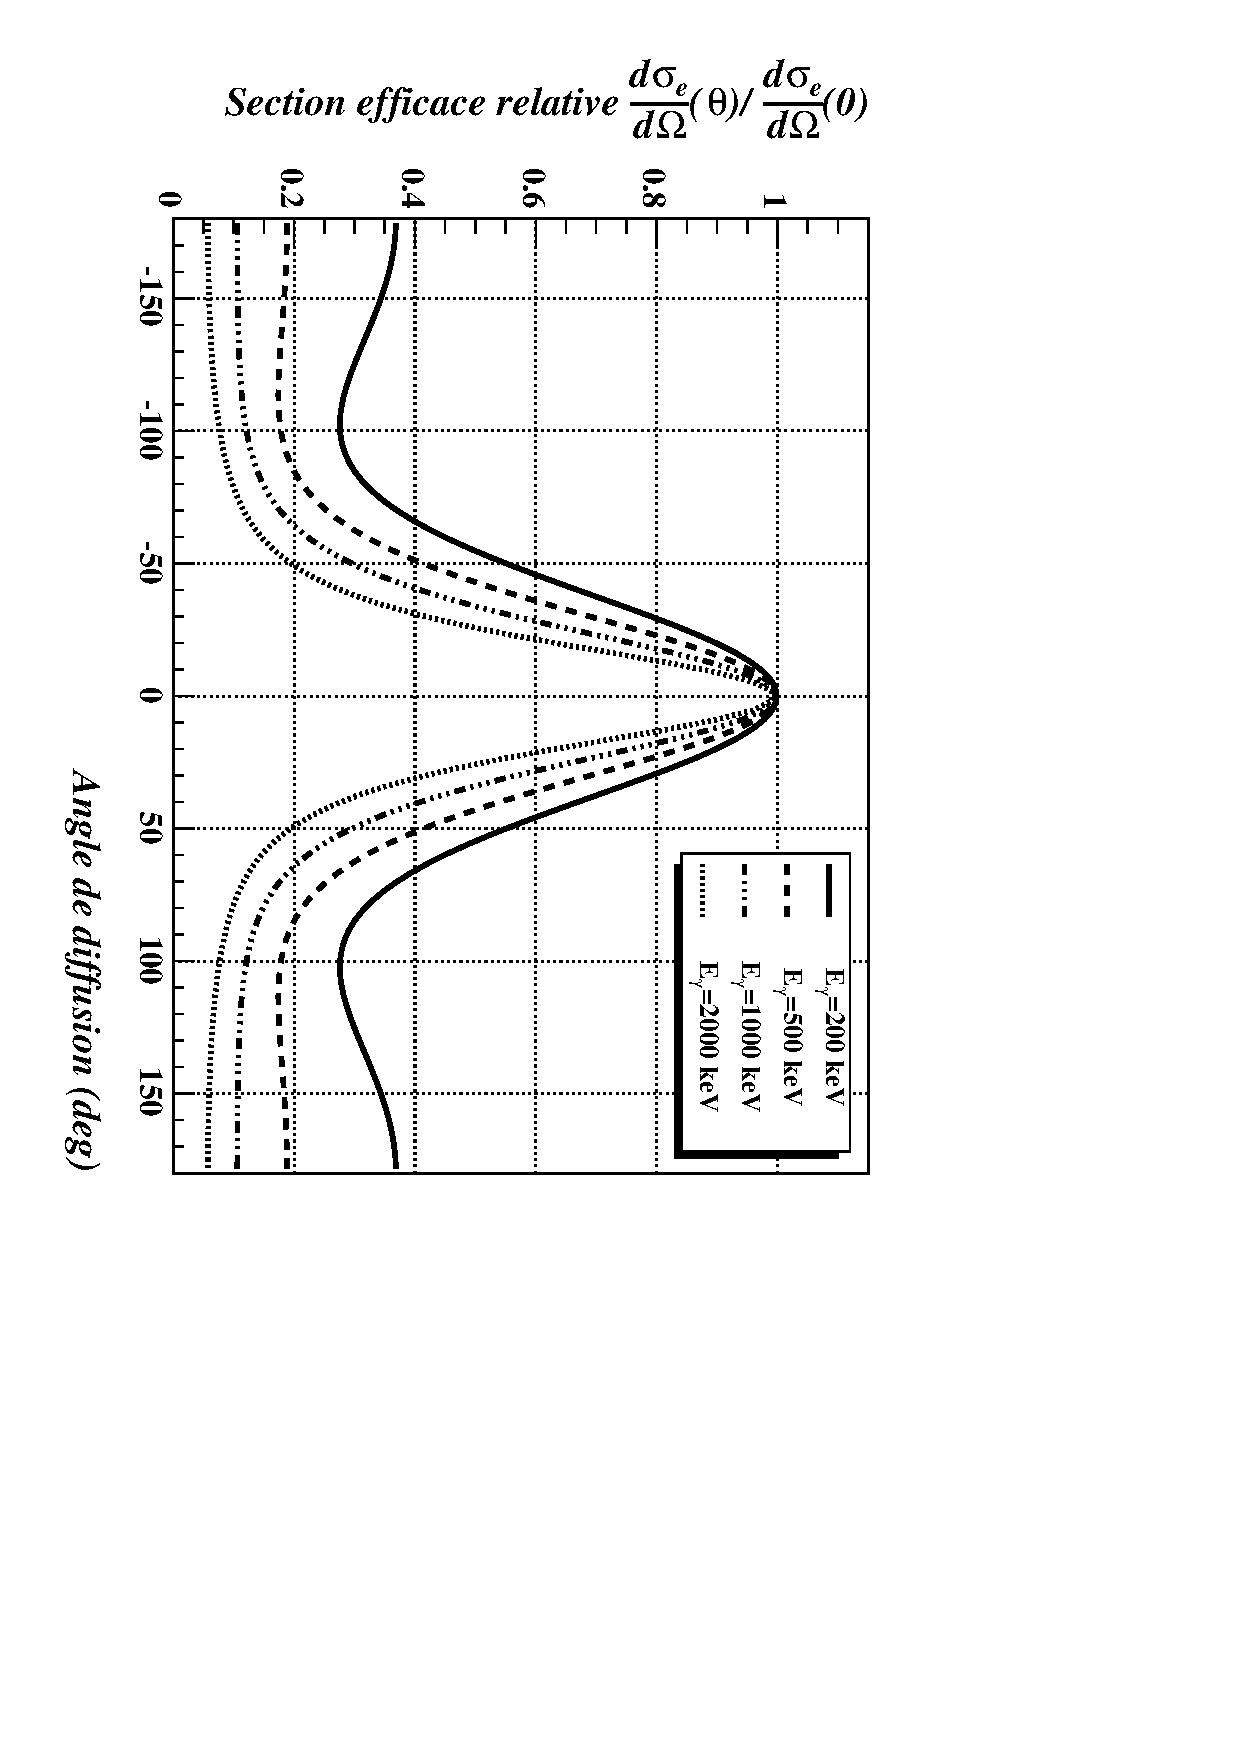
\includegraphics[height=0.8\textwidth,angle = 90.0 ]{figure/fig_cosolythuyet/klein.pdf}
\caption{Tán xạ Compton của các tia bức xạ $\gamma$ theo công thức Klein-Nishina cho khoảng năng lượng từ 200 keV đến 2 MeV.}
\label{fig:klein}
\end{figure}

\section{Hiệu ứng tạo cặp}

Ở mức năng lượng lớn hơn 1.022 MeV, xác suất của quá trình tạo cặp sẽ tăng dần và sẽ đạt giá trị lớn hơn giá trị xác suất của quá trình tán xạ Compton khi năng lượng của photon tới lớn hơn 8 MeV. Hiệu ứng tạo cặp gắn liền với hiện tượng biến đổi từ một tia bức xạ $\gamma$ thành một 		điện tử và một positron có động năng lần lượt là $T_{-}$ và $T_{+}$. Mối liên hệ giữa động năng của các hạt được tạo thành với năng lượng của photon ban đầu được biểu thị bằng công thức sau:

\begin{equation}
	h\nu_{0} = T_{-} + T_{+} + 2m_{0}c^{2}
\end{equation}

$h\nu_{0}$ là năng lượng của photon, $m_{0}$\nomenclature{$m$}{ Khối lượng điện tử} là khối lượng của một điện tử. Sự biến đổi trên chỉ có thể được thực hiện ở gần một hạt nhân hoặc gần một điện tử để đảm bảo định luật bảo toàn mô men động lượng được thỏa mãn. Tiết diện phản ứng của quá trình tạo cặp tỷ lệ với $Z^{2}$. Positron tạo thành từ phản ứng này sẽ hủy cặp với một điện tử khác để tạo ra hai tia bức xạ $\gamma$ có năng lượng 511 keV và được phát ra theo hai hướng đối lập.
	\clearHeading
	
	\chapter{Đối tượng và phương pháp nghiên cứu}
\label{ch:doituongnghiencuu}
\minitoc

%\newpage

\section{Một số loại detector}
\index{detector}

Trong Chương \ref{ch:tongquan} đã trình bày các nguyên lý ghi nhận bức xạ, trong phần này sẽ trình bày các phương pháp thực nghiệm để ghi nhận các tia $\gamma$

\begin{table}[!h]
\caption{So sánh một số detector}
\centering
\begin{tabular}{|c|c|c|c|}
\hline 
Loại Detector & Hệ thống điện tử & Thuật toán & sử dụng Trigger \\ 
\hline 
EUROBALL & analog & addback & có \\ 
\hline 
EXOGAM & analog & addback & có \\ 
\hline 
JUROGAM & analog + digital & không & không \\ 
\hline 
AGATA & digital & tracking $\gamma$ & trigger+triggerless \\ 
\hline 
\end{tabular} 
\label{table:detector}
\end{table}

Một detector ghi nhận $\gamma$ được thiết lập từ các detector nhỏ hơn trong đó mỗi detector nhỏ sẽ gồm các khối Germanium \nomenclature{Ge}{Germanium} được đặt trong một lớp bảo vệ. Các khối Germanium có thể được phân chia thành các vùng khác nhau  và mỗi vùng này sẽ được kết nối với một điện cực riêng. Trong phần này sẽ giới thiệu sơ lược về bốn loại detector khác nhau: EXOGAM, EUROBALL, JUROGAM và AGATA \cite{bib_Bazzaco, bib_Simpson} \nomenclature{AGATA}{ Advanced GAmma Tracking Array} với các thông số chính như trong Bảng \ref{table:detector}. Mỗi loại detector đều có những ưu điểm riêng, tuy nhiên detector AGATA cho phép ghi nhận các tia bức xạ  $\gamma$ với độ phân giải tốt nhất. Để có thể tái lập năng lượng của các tia bức xạ $\gamma$, thuật toán addback và tracking đã được sử dụng.

Các kết quả thực nghiệm sẽ được trình bày trong Chương \ref{ch:ketqua}.

\renewcommand\bibname{Tài liệu tham khảo chương \thechapter}
\bibliographystyle{ieeetr}
\bibliography{bibtex/biblio} %put path to the Bib from where the BibtexRun.bat is located 
	\clearHeading
		
	\chapter{Kết quả và thảo luận}
\label{ch:ketquaphantich}

\section{Các phương pháp phân tích số liệu}

Trình bày phương pháp phân tích số liệu. 

Có thể đưa các đoạn văn bản, công thức toán học, hình vẽ, bảng biểu, v.v., vào đây. Có thể bổ sung thêm các mục hoặc các tiểu mục khác thông qua lệnh section, subsection hay subsubsection v.v.

\section{Các kết quả chính}

\begin{figure}[!htb]
\centering
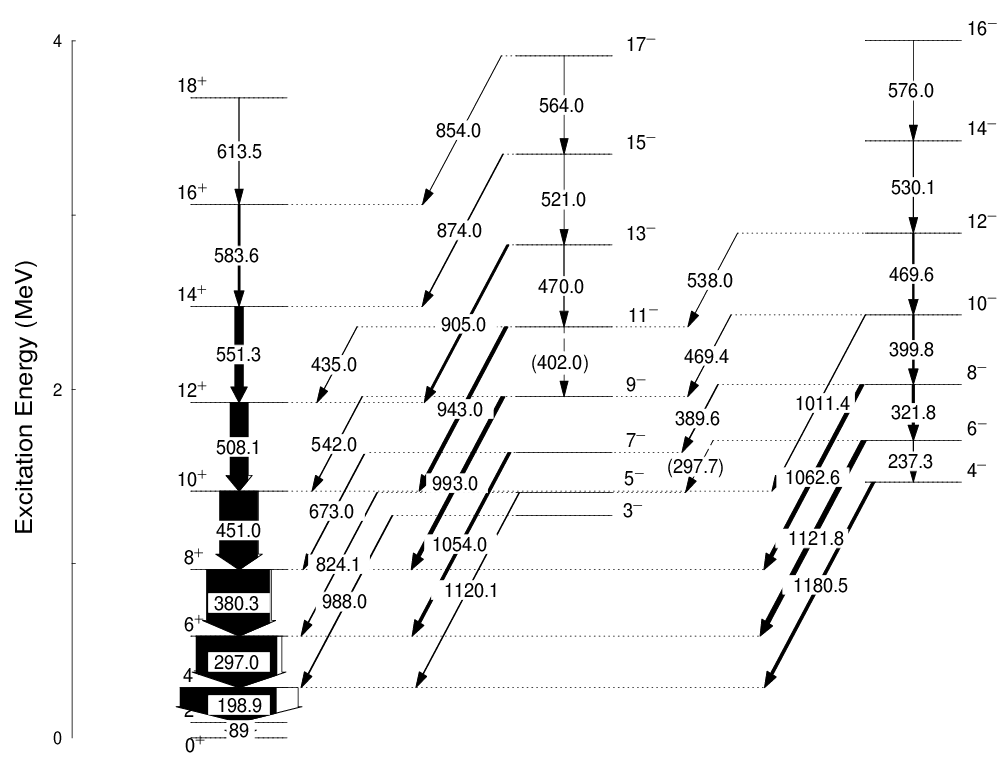
\includegraphics[width=0.4\textwidth]{figure/fig_ketquaphantich/156Gd.png}
\caption{Các mức năng lượng và tỷ lệ các chuyển dịch giữa các mức năng lượng của hạt nhân 156Gd được xác định bằng thực nghiệm.}
\label{fig:156Gd}
\end{figure} 

Trình bày các kết quả. 

Có thể đưa các đoạn văn bản, công thức toán học, hình vẽ, bảng biểu, v.v., vào đây. Có thể bổ sung thêm các mục hoặc các tiểu mục khác thông qua lệnh section, subsection hay subsubsection v.v.

Các mức năng lượng của hạt nhân 156Gd được thể hiện trên Hình \ref{fig:156Gd}.	
	\clearHeading

	\chapter*{Kết luận}
\label{ch:ketluan}
\addcontentsline{toc}{chapter}{Kết luận}
\makeatletter
	\markboth{\sl \@title}{\sl Kết luận}
\makeatother

Đưa ra các kết luận về các kết quả thu được, đề xuất các phương pháp thực nghiệm hoặc các phương pháp xử lý số liệu nếu cần v.v.

Có thể đưa các đoạn văn bản, công thức toán học, hình vẽ, bảng số v.v. vào đây. Có thể bổ sung thêm các mục hoặc các tiểu mục khác thông qua lệnh section, subsection hay subsubsection v.v.
	\clearHeading
	
\defbibheading{tiengViet}{ 
	\section*{Tài liệu tiếng Việt}
	\markboth{\sl Tài liệu tham khảo}{\sl Tài liệu tiếng Việt}
	\addcontentsline{toc}{section}{Tài liệu tiếng Việt}
}

\defbibheading{tiengAnh}{
	\section*{Tài liệu tiếng Anh}
	\markboth{\sl Tài liệu tham khảo}{\sl Tài liệu tiếng Anh}
	\addcontentsline{toc}{section}{Tài liệu tiếng Anh}
}

\printbibheading[heading=bibintoc, title = {Tài liệu tham khảo}] 
\printbibliography[heading=tiengViet, keyword=VN]
\printbibliography[heading=tiengAnh, keyword=EN]
\clearHeading

\renewcommand{\appendixtocname}{Phụ lục}
\addappheadtotoc
\renewcommand{\chaptername}{\appendixname}

\appendix
	\chapter{Phổ gamma từ các detector khác nhau}
\label{phuluc:cacdothi}

\section{Các phổ gamma từ detector EUROBALL} 
Trong phần này trình bày tất cả các kết quả thực nghiệm, các thí nghiệm, các đồ thị thu được trong quá trình làm thực nghiệm v.v. Phần này được sử dụng để dẫn chiếu.

\section{Các phổ gamma từ detector JUROGAM}
Trong phần này trình bày tất cả các kết quả thực nghiệm, các thí nghiệm, các đồ thị thu được trong quá trình làm thực nghiệm v.v. Phần này được sử dụng để dẫn chiếu.
	\clearHeading
	\chapter{Các số liệu thực nghiệm}
\label{phuluc:solieuthucnghiem}

\section{Số liệu thực nghiệm từ detector EUROBALL} 
Trong phần này trình bày tất cả các kết quả thực nghiệm, các thí nghiệm, các đồ thị thu được trong quá trình làm thực nghiệm, v.v. Phần này được sử dụng để dẫn chiếu.

\section{Số liệu thực nghiệm từ detector JUROGAM}
Trong phần này trình bày tất cả các kết quả thực nghiệm, các thí nghiệm, các đồ thị thu được trong quá trình làm thực nghiệm, v.v. Phần này được sử dụng để dẫn chiếu.


	\clearHeading
     
\end{document}